\documentclass{VUMIFSlides}
\usepackage{times}
\usepackage[T1]{fontenc}
\usepackage{color}
\usepackage{verbatim}
\usepackage{graphicx}
\usepackage{fancyvrb}
\usepackage{bm}
\usepackage{amsfonts}
\usepackage{float}
\usepackage{hyperref}
\usepackage{textpos} % FOR LOGO
\usepackage[english,lithuanian]{babel}
\usepackage{animate}
\usepackage{caption} 
\usepackage{subfig}

\hypersetup{
    pdfauthor=Justas Baniulis,
    linktoc=all,     %set to all if you want both sections and subsections linked
}

\title[Ligų aptikimas naudojant plaučių echoskopiją]{Ligų aptikimas naudojant plaučių echoskopiją}
\subtitle{Kursinio darbo pristatymas}
\author[Justas Baniulis]{\texorpdfstring{Autorius: Justas Baniulis \\ Vadovas: asist. dr. Tomas Plankis}{Autorius: Justas Baniulis, Vadovas: asist. dr. Tomas Plankis}} 
\institute[MIF PS]{Vilniaus universitetas \\
Matematikos ir informatikos fakultetas \\
Informatikos institutas \\
Programų sistemų bakalauro studijų programa}
\date[2023-01-22]{2023-01-22}

\bibliography{bib}

% Let's get started
\begin{document}

\begin{frame}
  \maketitle
\end{frame}

\begin{frame}{Įžanga}{}
    {\bf Plaučių echoskopija}
    \begin{itemize}
        \item Tyrimas, kuris vizualizuoja plaučių artefaktus naudojantis aukšto garso bangomis.\\ (\ref{img:plauciai_art} pav.)
    \end{itemize}
    \begin{figure}[H]
    \centering
    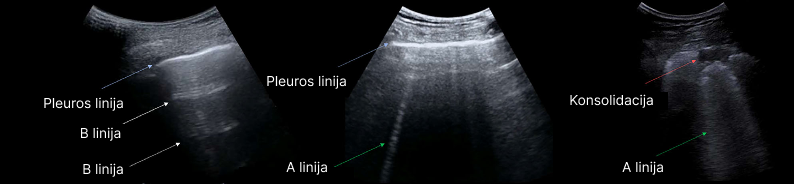
\includegraphics[scale=0.5]{img/plauciai_artefaktai.png}
    \caption{Plaučių artefaktų pavyzdžiai \cite{demi2023new}}
    \label{img:plauciai_art}
\end{figure}
\end{frame}

\begin{frame}[c]{Įžanga}{}
    \begin{itemize}
        \item Pagal artefaktus medikai nustato diagnozes. (\ref{tab:ligos} lentelė)
        \item Patrauklus naudojimui medicinoje, nes pigesnis, patogesnis ir saugesnis už kitus plaučių tyrimus 
        \cite{demi2023new}
    \end{itemize}

    \begin{table}[H]\footnotesize
  \centering
  \caption{Echoskopijos artefaktų ir ligų sąryšis \cite{demi2023new, cammarota2023lung}}
  \begin{tabular}{|l|c|c|c|c|c|} \hline
     Artefaktas & Galimos diagnozės \\
    \hline
    A linija  & Sveiki plaučiai \\
    B linija & Širdies ydos, COVID-19, virusinis plaučių uždegimas, plaučių edema \\
    Konsolidacija & Bakterinis plaučių uždegimas, atelektazė, plaučių sumušimas \\
    Pleuros linija & Pneumotoraksas, pleuros efuzija, pleuros fibrozė \\
    \hline
  \end{tabular}
  \label{tab:ligos}
\end{table}
\end{frame}

\begin{frame}[c]{Motyvacija, tikslas, uždaviniai}{}
    {\bf Darbo motyvacija}
    \begin{itemize}
        \item Medikams išmokti interpretuoti echoskopijos nuotraukas yra sunku, užtrunka laiko ir žmogiškųjų išteklių. Padėti gali dirbtinis intelektas \cite{cammarota2023lung}.
    \end{itemize}
    
    \vspace{0.35 cm}
    {\bf Darbo tikslas}
    \begin{itemize}
        \item Apžvelgti ir palyginti giliojo mokymosi tinklus, kurie nustato diagnozę iš plaučių echoskopijos.
    \end{itemize}
    
    \vspace{0.35 cm}
    {\bf Darbo uždaviniai}
    \begin{itemize}
        \item Apžvelgti transformerių neuroninio tinklo sprendimą.
        \item Apžvelgti „Fuzzy pooling“ neuroninio tinklo sprendimą.
        \item Apžvelgti ilgos trumpalaikės atminties neuroninio tinklo sprendimą.
        \item Sukurti adaptuotus eksperimentinius modelius.
    \end{itemize}
\end{frame}

\begin{frame}[c]{Sprendimai literatūroje}{}
    {\bf Transformerių \cite{PAY21}}
    \begin{itemize}
        \item Regos transformerių neuroninis tinklas („ViT“) su „Linformer“ enkoderiu.
        \item Standartizavo visas nuotraukas ir naudojo parametrų balansavimo mechanizmą.
    \end{itemize}
    \vspace{0.3cm}
    {\bf „Fuzzy pooling“ (angl. neapibrėžto sutelkimo) \cite{HASAN2023}}
    \begin{itemize}
        \item VGG, ResNet ir Xception architektūroms pritaikyti neapibrėžto sutelkimo sluoksniai, naudojantys neapibrėžtąją logiką.
        \item Modeliai su apkeistu paskutiniu ir visais apkeistais sutelkimo sluoksniais. 
        \item Triukšmas nuotraukose pašalintas su kontrasto pakeitimais ir erdviniu filtravimu. 
    \end{itemize}
    \vspace{0.3cm}
    {\bf Ilgos trumpalaikės atminties \cite{LSTM}}
    \begin{itemize}
        \item Apmokyti 68 modeliai su paskutiniu ilgos trumpalaikės atminties sluoksniu vaizdo įrašams.
        \item 5, 10, 15 ir 20 kadrų išgavimo iš vaizdo įrašų konfigūracijos.
    \end{itemize}
\end{frame}

\begin{frame}[c]{Sprendimai literatūroje}{}
{\bf Visi autoriai:}
\begin{itemize}
        \item Naudojosi POCUS duomenų rinkiniu \cite{born2021accelerating}. Vaizdo įrašai ir nuotraukos surinkti ir sužymėti medikų.
        \item Klasifikavo COVID-19, bakterinio uždegimo ir sveikų plaučių klases - jų daugiausiai yra šiame rinkinyje.
\end{itemize}
\end{frame}

\begin{frame}[c]{Eksperimentinė dalis}    
    \begin{itemize}
        \item  Adaptuoti MobileNetV3Small, NASNetMobile, ConvNeXtTiny  CNN modeliai - orientuotasi į efektyvumą.
        \item  POCUS duomenų rinkinys.
        \item  Klasifikuoja COVID-19, bakterinio plaučių uždegimo, virusinio plaučių uždegimo ir sveikų plaučių klases.
        \item  Virusinio uždegimo klasė turi labai mažai nuotraukų - tik 72. COVID-19 apie 500 nuotraukų, sveikų plaučių apie 1000...
        \item  Apmokymui naudota židinio nuostolių funkcija ir apskaičiuoti klasių svoriai, kad išspręsti klasių disbalansą. 
    \end{itemize}
\end{frame}

\begin{frame}[c]{Rezultatai}
    % Left side: List
    \begin{minipage}[c]{0.45\textwidth}
        \begin{itemize}
            \item Geriausias tikslumas - Xception su visais neapibrėžto sutelkimo sluoksniais
            \item Aukščiausia precizija - „POCFormer“ uždegimo ir sveikų plaučių, Xception-LSTM ir ConvNeXtTiny
            \item Aukščiausią specifiškumas - Xception-LSTM, „POCFormer“ COVID-19 ir sveikų plaučių, MobileNetV3Small ir ConvNeXtTiny modeliai.
        \end{itemize}
    \end{minipage}
    % Right side: Image
    \hfill
    \begin{minipage}[c]{0.45\textwidth}
        \begin{figure}[H]
            \centering
            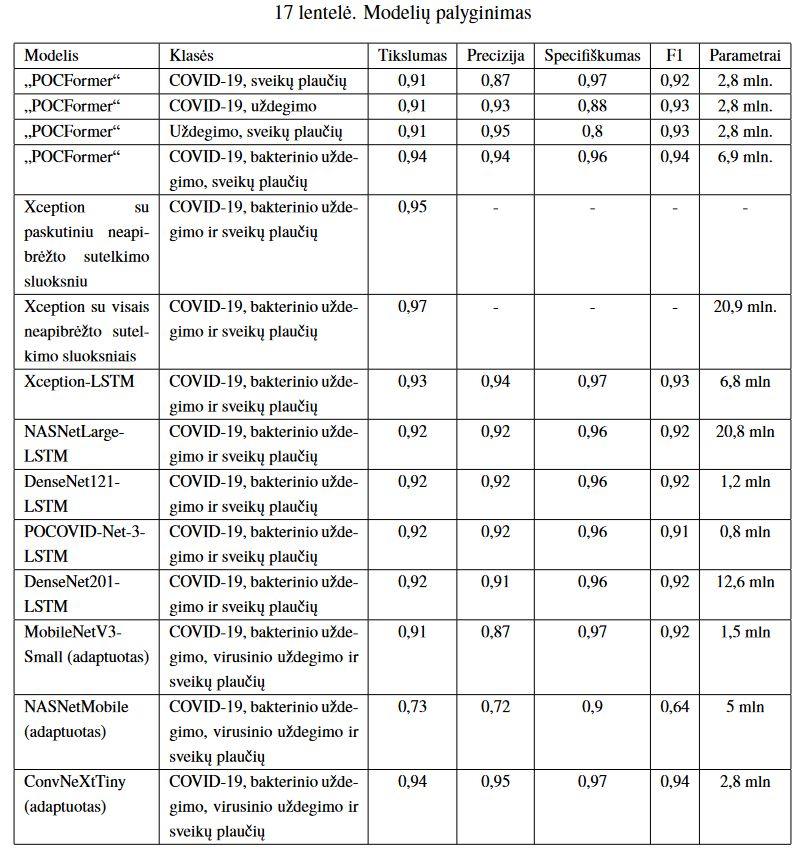
\includegraphics[scale=0.33]{img/Capture.JPG}
            \label{img:POCFormer}
        \end{figure}
    \end{minipage}
\end{frame}

\begin{frame}[c]{Rezultatai}
    % Left side: List
    \begin{minipage}[c]{0.45\textwidth}
        \begin{itemize}
            \item Aukščiausias F1 - „POCFormer“ daugelio klasių ir ConvNeXtTiny.
            \item Mažiausia parametrų - POCOVID-Net-3-LSTM.
            \item Sunku palyginti modelius dėl skirtingų pateikiamų metrikų.
        \end{itemize}
    \end{minipage}
    % Right side: Image
    \hfill
    \begin{minipage}[c]{0.45\textwidth}
        \begin{figure}[H]
            \centering
            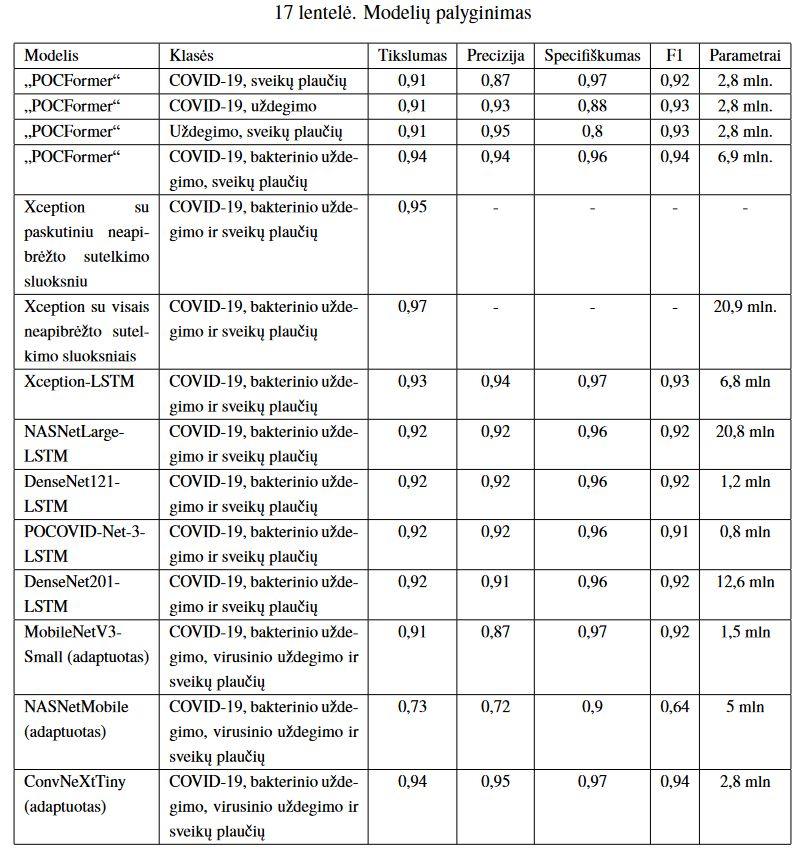
\includegraphics[scale=0.33]{img/Capture.JPG}
            \label{img:POCFormer}
        \end{figure}
    \end{minipage}
\end{frame}

\begin{frame}[c]{Išvados ir rekomendacijos}{}
    {\bf Išvados:}
    \begin{itemize}
        \item Darbe apžvelgti transformerių, „Fuzzy pooling“ ir ilgos trumpos atminties ir du eksperimentiniai modeliai turi aukštas metrikas - visos yra intervale tarp 0,8 ir 0,97.
        \item Aptimkamos tik 2-3 plaučių ligos - gali būti nepatrauklu medikams.
        \item POCUS duomenų rinkinyje trūksta kitų ligų.
        \item Modeliai turi didelius parametrų kiekius - svarbu mobiliems prietaisams.
    \end{itemize}
    \vspace{0.5cm}
    {\bf Rekomendacijos:}
        \begin{itemize}
        \item Papildyti duomenų rinkinius kitomis ligomis.
        \item Pamažinti parametrų kiekį, kad veikimas būtų efektyvesnis su labai ribotais resursais.
    \end{itemize}
\end{frame}


% Bibliography
\begin{frame}[allowframebreaks]{Šaltiniai}
    \printbibliography 
\end{frame}

 \begin{frame}
  \maketitle
\end{frame}
% \appendix

\end{document}
